\documentclass[paper=a4, fontsize=11pt]{article} 
\usepackage[top=1in, bottom=1in, left=1in, right=1in]{geometry}
\usepackage{amstext}
\usepackage{subfigure}
\RequirePackage{graphicx}
\RequirePackage{longtable,multirow,hhline,tabularx,array}
\usepackage[english]{babel} 
\usepackage{CJKutf8}
\usepackage{indentfirst}
\RequirePackage{colortbl,booktabs}
\linespread{1.5}

\title{
\normalfont \normalsize
\huge Battle of Online and Offline Consumption: \\
Comparative Analysis of Amazon and Walmart Stocks
}
\author{Cai Yuzhu, Li Hongchi, Ning Xu, Xue Zheng}
\date{\normalsize\today}

\begin{document}
\maketitle

%%%%%%%%%%%%%%%%%%%%%%   Introduction   %%%%%%%%%%%%%%%%%%%%%%%
\section{Introduction}
Online consumption is a relative new and prevailing concept raised in recent decade. Amazon is arguably one of the most successful online firms. As of this writing, its market cap is over \$460 billion, almost twice than the large and well-known offline retailer, Wal-Mart's, with market cap about \$240 billion.

Amazon, as a business model, has many potential advantages relative to a physical operation. It held out the potential of lower inventory and distribution costs and reduced overhead. Consumers could find the books products they were looking for more easily and a broader variety could be offered for sale in the first place. It could accept and fulfill orders from almost any domestic location with equal ease. And most purchases made on its site would be exempt from sales tax.

On the other hand, it is also acknowledged that there are some limitations of online operations. Customers would have to wait for their orders to be received, processed, and shipped. Because they couldn't physically inspect a product before ordering, Amazon would have to make its returns and redress processes transparent and reliable, and offer other ways for consumers to learn as much about the product as possible before buying.

The task to judge the performance of online consumption against offline consumption is compelling. And the methods of judgments comparisons can be diverged. In this term paper, our group conducts time series data models with conditional heteroscedasticity, which are widely applied in financial data analysis, to depict the stock volatility of Amazon and Wal-Mart's.

The historical stock price data presents a diverged trend that seems to reveal a competitive relation between Amazon and Wal-Mart. Admittedly the share price cannot represent complete information about the firms, such as market shares. Nevertheless, this is a direct and prevalent way to evaluate firms' performance through numerical results. And the maximize likelihood method (MLE) estimations will also provide helpful suggestions about their prospective performance.

We organize our discussion as follows. The next section lays out some basic facts about the historical stock price data: statistics and time plots. Section 3 discusses how to determine the specifications of models. Section 4 conducts MLE method to estimate the parameters of models. Section 5 explores future performance and compares our prediction with recent data. A short concluding section follows.

%%%%%%%%%%%%%%%%%%%%%%   Data Processing   %%%%%%%%%%%%%%%%%%%%%%%
\section{Data Processing}
In our research report, we use Walmart as the representative of offline retail industry and Amazon as that of online retail industry. We focus on the daily log return of Walmart stock and Amazon stock from January 3th, 2010 to December 30th, 2016, with 1761 observations. All the data are pulled from Wind Terminal.

We compute the daily log return based on the  daily close price. Let $r_t$ be the log return of an asset at time $t$, and the formula we use to calculate the log return is
\[ r_t = ln(\frac{p_t}{p_{t-1}}) \times 100\% \]
where $p_t$ is the close price in day $t$ and $p_{t-1}$ is the close price in day {t-1}.

The descriptive statistics and time plots are shown in Table \ref{ds} and Figure \ref{tp}.

\begin{table}[!htbp]
\caption{Descriptive Statistics}  
\centering  
\subtable[Amazon Stock]
{  
\begin{tabular}{ccccc}
  \toprule
  \rowcolor[gray]{.8}
Year & Sample & Mean(\%) & Sd(\%) \\ 
  \midrule
2010 & 251 & 0.1179 & 2.0591 \\ 
2011 & 252 & -0.0155 & 2.4337 \\ 
2012 & 250 & 0.1484 & 1.9656 \\ 
2013 & 252 & 0.1839 & 1.6947 \\ 
2014 & 252 & -0.0995 & 2.0677 \\ 
2015 & 252 & 0.3089 & 2.0582 \\ 
2016 & 252 & 0.0412 & 1.8682 \\ 
2010-2016 & 1761 & 0.0978 & 2.0323 \\ 
   \bottomrule
\end{tabular}
}  
\qquad  
\subtable[Walmart Stock]
{          
\begin{tabular}{ccccc}
  \toprule
  \rowcolor[gray]{.8}
Year & Sample & Mean(\%) & Sd(\%) \\ 
  \midrule
2010 & 251 & 0.0068 & 0.8782 \\ 
2011 & 252 & 0.0515 & 1.0469 \\ 
2012 & 250 & 0.0627 & 1.0309 \\ 
2013 & 252 & 0.0662 & 0.7749 \\ 
2014 & 252 & 0.0445 & 0.8367 \\ 
2015 & 252 & -0.1229 & 1.3191 \\ 
2016 & 252 & 0.0590 & 1.2030 \\ 
2010-2016 & 1761 & 0.0239 & 1.0297 \\ 
   \bottomrule
\end{tabular}
}
\label{ds} 
\end{table}  

\begin{figure}[!htbp]
\begin{minipage}[!htbp]{0.5\linewidth}
\centering
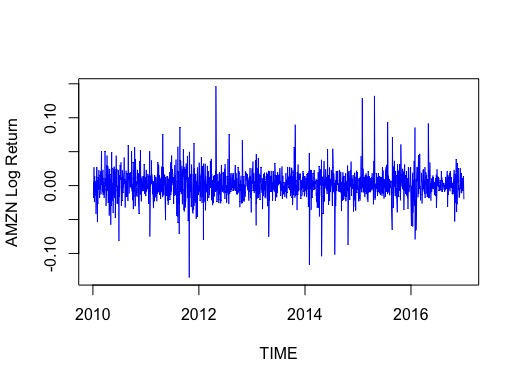
\includegraphics[scale = 0.45]{img/timeplot_AMZN}
\end{minipage}
\begin{minipage}[!htbp]{0.5\linewidth}
\centering
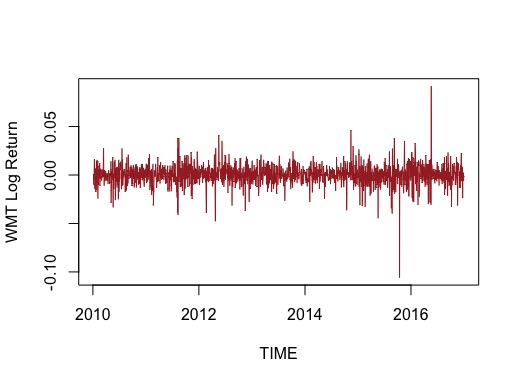
\includegraphics[scale = 0.45]{img/timeplot_WMT}
\end{minipage}
\caption{Timeplots of Amazon (Blue) and Walmart (Red) Stocks}
\label{tp}
\end{figure}

From Table \ref{ds}, we can see that the average log return of Amazon stock  is four times greater than Walmart stock, while the log return of Walmart stock is more stable than Amazon's. From the timeplots in Figure \ref{tp}, the log return series for both stocks appear to be relatively stationary over times, fluctuating around the mean value.

%%%%%%%%%%%%%%%%%%%%%  Model Establishment   %%%%%%%%%%%%%%%%%%%%%%
\section{Model Establishment}
\subsection{Model Specification}
First of all, we determine the model to capture the log return fluctuation of Amazon stock. Figure \ref{cf_AMZN}.(a) shows the sample ACF of the log returns, which suggests that there is no significant serial correlations and the series is stationary. Observing the squared log returns for Amazon stock in Figure \ref{cf_AMZN}.(c) we find that the log returns are not serially correlated but dependent, which indicates the ARCH effect in the return series. Similar results can also be found for Walmart stock in Figure \ref{cf_WMT} that there also exists an ARCH effect in Walmart's return series.

\begin{figure}[!htbp]
\centering
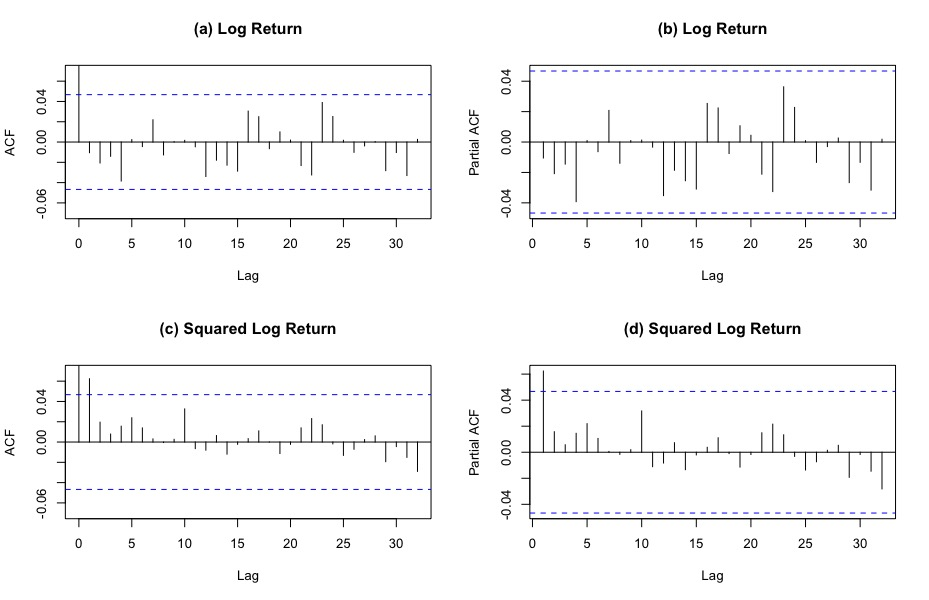
\includegraphics[width = 5in]{img/cf_AMZN}
\caption{ACF and PACF of Amazon Stock}
\label{cf_AMZN}
\end{figure}

\begin{figure}[!htbp]
\centering
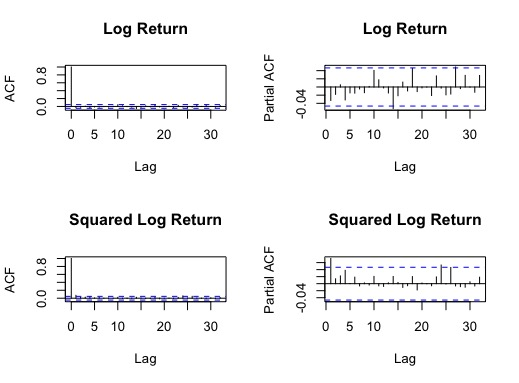
\includegraphics[width = 5in]{img/cf_WMT}
\caption{ACF and PACF of Walmart Stock}
\label{cf_WMT}
\end{figure}

\subsection{Mean Equation}
According to the Figure \ref{cf_AMZN}.(b), the daily log returns of Amazon stock follow an ARMA(0,0) model because there is no cutoff in the PACF of log return. Therefore, we propose a mean equation that is simply a constant plus innovations, $r_t = \mu + a_t$, where $r_t$  is the log return of an asset at time $t$, $\mu$ is the estimate of mean log return. 

The $a_t^2$ series is then used to check for conditional heteroscedasticity (ARCH effects). To consolidate the observation results in Figure \ref{cf_AMZN}.(c), the ARCH effect exists in log return series, we perform the Ljung–Box statistics Q(m) to the $\{a_t^2\}$ series. The null hypothesis is that the first m lags of ACF of the $a_t^2$ series are zero. The results of Ljung–Box test shows an ARCH effect exists in this log return series with Q(5) = 9.6519, the p-value of which is close to zero.

Using the same method above to analyze the ACF and PACF of WMT log returns shown in Figure \ref{cf_WMT}, we conclude that the WMT log returns' mean equation is also an ARMA(0,0) process. And there exists an ARCH effect in WMT's log return series. Although someone may argue that Figure \ref{cf_WMT} shows significant correlation at lag-14 and lag-27, the EACF results in Table \ref{eacf_WMT} provide the evidence that ARMA(0,0) is proper. 

\begin{table}[!htbp] \centering 
  \caption{EACF of Log Returns of Walmart Stock} 
  \label{eacf_WMT} 
\begin{tabular}{c|cccccccccccccc} 
\hline 
\hline
AR/MA & 0 &1 & 2 & 3 & 4 & 5 & 6 & 7 & 8 & 9 & 10 & 11 & 12 & 13\\
\hline 
0 & o & o & o & o & o & o & o & o & o & o & o & o & o & x \\ 
1 & x & o & o & o & o & o & o & o & o & o & o & o & o & o \\ 
2 & x & x & o & o & o & o & o & o & o & o & o & o & o & o \\ 
3 & x & x & x & o & o & o & o & o & o & o & o & o & o & o \\ 
4 & x & x & x & x & o & o & o & o & o & o & o & o & o & o \\ 
5 & x & x & x & x & x & o & o & o & o & o & o & o & o & o \\ 
6 & x & x & x & o & x & x & o & o & o & o & o & o & o & o \\ 
7 & x & x & o & x & x & x & x & o & o & o & o & o & o & o \\ 
\hline
\end{tabular} 
\end{table} 

\subsection{Volatility Equation}
Based on the Figure \ref{cf_AMZN}.(d), there is a sudden cutoff at lag-1 squared $a_t$. Hence, we entertain an ARCH(1) model and a GARCH(1,1) model for the volatility and we specify the model as the following:
\[ r_t = \mu+a_t, a_t = \sigma_t \epsilon_t \]
\[ \text{ARCH(1): } \sigma_t^2 = \alpha_0+\alpha_1 a_{t-1}^2 \]
\[ \text{GARCH(1,1): } \sigma_t^2= \alpha_0+\alpha_1 a_{t-1}^2+\beta_1 \sigma_{t-1}^2 \]
in which $\epsilon_t$, we assume as a Gaussian innovation that is independent and identically distributed follows a Normal distribution with mean zero and variance one.

Similar results will be derived for the log return series of Walmart stock. We entertain an ARCH(4) model and a GARCH(1,1) model as the alternative volatility equations:
\[ r_t = \mu+a_t, a_t = \sigma_t \epsilon_t \]
\[ \text{ARCH(4): } \sigma_t^2 = \alpha_0+\alpha_1 a_{t-1}^2+\alpha_2 a_{t-2}^2+\alpha_3 a_{t-3}^2+\alpha_4 a_{t-4}^2 \]
\[ \text{GARCH(1,1): } \sigma_t^2= \alpha_0+\alpha_1 a_{t-1}^2+\beta_1 \sigma_{t-1}^2 \]
where $\epsilon_t \sim N(0,1)$.


%%%%%%%%%%%%%%%%%%%   Comparison & Estimation   %%%%%%%%%%%%%%%%%%%%
\section{Estimation Analysis}
\subsection{Estimation and Model comparison}
To determine the more adequate model for Amazon stock, we perform the Ljung-Box test for the standardized residuals and the squared standardized residuals. However, there is no evident difference between ARCH(1) model and GARCH(1,1) model according to the test results in Table \ref{lb_AMZN}. Then we use log likelihhod and information criteria to compare models and derive the estimation results in Table \ref{est_AMZN}.

\begin{table}[!htbp] \centering 
  \caption{Ljung-Box tests for ARCH(1) and GARCH(1,1) models for AMZN Stock} 
  \label{lb_AMZN} 
\begin{tabular}{cc|cccccc} 
\\[-1.8ex]\hline 
\hline
& & \multicolumn{3}{c}{Standardized residuals} & \multicolumn{3}{c}{Squared standardized residuals} \\
& & Q(10) & Q(15) & Q(20) & Q(10) & Q(15) & Q(20) \\
\hline 
\multirow{2}{*}{ARCH(1)} & statistic & 4.7873 & 10.2395 & 12.8693 & 3.9721 & 4.7376 & 5.1054 \\
& p-value & 0.9049 & 0.8044 & 0.8829 & 0.9486 & 0.9941 & 0.9997 \\
\multirow{2}{*}{GARCH(1,1)} & statistic & 4.1734 & 10.2365 & 12.8473 & 3.0443 & 4.2163 & 4.7107 \\
& p.value & 0.9392 & 0.8046 & 0.8838 & 0.9804 & 0.9969 & 0.9999 \\
\hline
\hline 
\end{tabular} 
\end{table} 

\begin{table}[!htbp] \centering 
  \caption{Results of Estimation of Two Volatility Models for AMZN Stock} 
  \label{est_AMZN} 
\begin{tabular}{@{\extracolsep{5pt}}lcc} 
\\[-1.8ex]\hline 
\hline
 & ARCH(1) & GARCH(1,1) \\ 
 $\mu$ & 0.115$^{**}$ & 0.137$^{***}$ \\ 
  & (0.046) & (0.046) \\ 
 $\alpha_0$ & 3.515$^{***}$ & 1.020$^{***}$ \\ 
  & (0.149) & (0.344) \\ 
 $\alpha_1$ & 0.168$^{***}$ & 0.129$^{***}$ \\ 
  & (0.036) & (0.032) \\ 
 $\beta_1$ &  & 0.637$^{***}$ \\ 
  &  & (0.098) \\ 
\hline \\[-1.8ex] 
Observations & 1761 & 1761 \\ 
Log Likelihood & -3724.855 & -3720.010 \\ 
Akaike Inf. Crit. & 4.234 & 4.229 \\ 
Bayesian Inf. Crit. & 4.243 & 4.242 \\ 
\hline 
\hline \\[-1.8ex] 
\textit{Note:}  & \multicolumn{2}{r}{$^{*}$p$<$0.1; $^{**}$p$<$0.05; $^{***}$p$<$0.01} \\ 
\end{tabular} 
\end{table} 

Based on the results in Table \ref{est_AMZN}, GARCH(1,1) model is more appropriate because it has the largest value of Log Likelihood and the smallest value of AIC and BIC. And all estimated parameters are highly significant under 1\% significance level.

Consequently, we propose an ARMA(0,0)+GARCH(1,1) model to depict the log return series of Amazon stock:
\[ r_t = 0.137+a_t\]
\[ a_t = \sigma_t \epsilon_t, \epsilon_t \sim N(0,1) \]
\[ \sigma_t^2 = 1.02+0.129a_{t-1}^2+0.637\sigma_{t-1}^2 \]

\begin{table}[!htbp] \centering 
  \caption{Ljung-Box tests for ARCH(4) and GARCH(1,1) models for WMT Stock} 
  \label{lb_WMT} 
\begin{tabular}{cc|cccccc} 
\\[-1.8ex]\hline 
\hline
& & \multicolumn{3}{c}{Standardized residuals} & \multicolumn{3}{c}{Squared standardized residuals} \\
& & Q(10) & Q(15) & Q(20) & Q(10) & Q(15) & Q(20) \\
\hline 
\multirow{2}{*}{ARCH(4)} & statistic & 9.6623 & 15.0804 & 19.5692 & 1.4971 & 1.9193 & 3.6344 \\
& p-value & 0.4706 & 0.4456 & 0.4852 & 0.9989 & 0.9999 & 0.9999 \\
\multirow{2}{*}{GARCH(1,1)} & statistic & 8.8064 & 14.4575 & 18.5378 & 1.6428 & 1.9398 & 4.0184 \\
& p.value & 0.5506 & 0.4912 & 0.5520 & 0.9984 & 0.9999 & 0.9999 \\
\hline
\hline 
\end{tabular} 
\end{table} 

\begin{table}[!htbp] \centering 
  \caption{Results of Estimation of Two Volatility Models for WMT Stock} 
  \label{est_WMT} 
\begin{tabular}{@{\extracolsep{5pt}}lcc} 
\\[-1.8ex]\hline 
\hline
 & ARCH(4) & GARCH(1,1) \\ 
  $\mu$ & 0.024 & 0.033 \\ 
  & (0.023) & (0.024) \\ 
 $\alpha_0$ & 0.773$^{***}$ & 0.442$^{**}$ \\ 
  & (0.042) & (0.187) \\ 
 $\alpha_1$ & 0.130$^{***}$ & 0.140$^{***}$ \\ 
  & (0.035) & (0.040) \\ 
 $\alpha_2$ & 0.000 &  \\ 
  & (0.018) &  \\ 
 $\alpha_3$ & 0.034 &  \\ 
  & (0.024) &  \\ 
 $\alpha_4$ & 0.112$^{***}$ &  \\ 
  & (0.040) &  \\ 
 $\beta_1$ &  & 0.445$^{**}$ \\ 
  &  & (0.207) \\ 
\hline \\[-1.8ex] 
Observations & 1761 & 1761 \\ 
Log Likelihood & -2498.390 & -2506.020 \\ 
Akaike Inf. Crit. & 2.844 & 2.851 \\ 
Bayesian Inf. Crit. & 2.863 & 2.863 \\ 
\hline 
\hline \\[-1.8ex] 
\textit{Note:}  & \multicolumn{2}{r}{$^{*}$p$<$0.1; $^{**}$p$<$0.05; $^{***}$p$<$0.01} \\ 
\end{tabular} 
\end{table} 

Following the same logic above and combining the results in Table \ref{lb_WMT} and Table \ref{est_WMT}, the ARCH(4) model is more adequate for volatility in log returns of Walmart stock. Thus, we propose an ARMA(0,0)+ARCH(4) model to depict the log return series of Walmart stock:
\[ r_t = 0.024+a_t\]
\[ a_t = \sigma_t \epsilon_t, \epsilon_t \sim N(0,1) \]
\[ \sigma_t^2 = 0.773+0.13a_{t-1}^2+0.034a_{t-3}^2+0.112a_{t-4}^2 \]

For each model mentioned above, we also estimated a similar one with a innovation that follows a student-t distribution correspondingly. All the models with student-t innovations have adequate mean and volatility equations, but when we concern the values of their log likelihood, AIC and BIC, we find that they are less appropriate than their counterparts, the ones with normal innovations. So we will still use the models with normal innovation assumption for further estimation. 

\subsection{Results Analysis}
Figure \ref{vol_stdr_amzn} shows the estimated volatility process and the standardized shocks for the log return series of Amazon stock based on the proposed GARCH(1,1) model.

\begin{figure}[!htbp]
\begin{minipage}[!htbp]{0.5\linewidth}
\centering
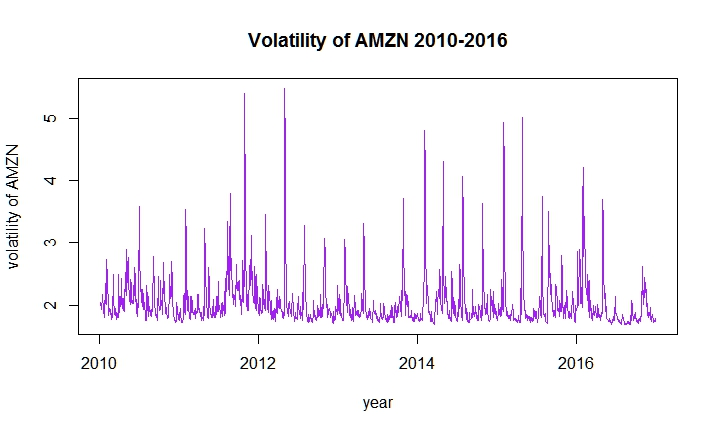
\includegraphics[scale = 0.45]{img/vol_AMZN}
\end{minipage}
\begin{minipage}[!htbp]{0.5\linewidth}
\centering
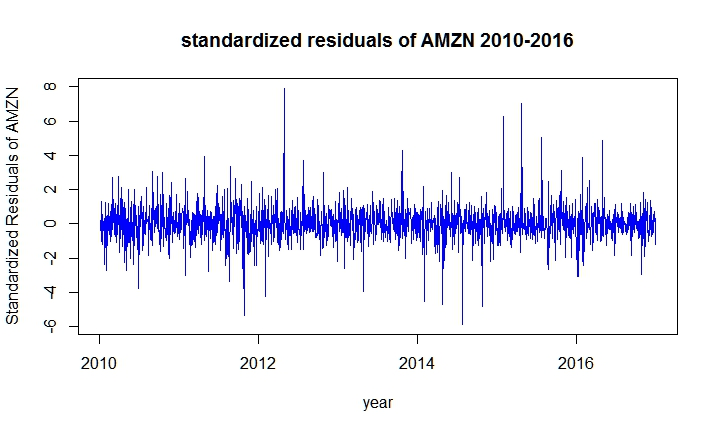
\includegraphics[scale = 0.45]{img/stdr_AMZN}
\end{minipage}
\caption{Estimated Volatility Process and Standardized Shocks for AMZN}
\label{vol_stdr_amzn}
\end{figure}

Figure \ref{vol_stdr_wmt} shows the estimated volatility process and the standardized shocks for the log return series of Walmart stock based on the proposed ARCH(4) model. The volatility denotes the conditional standard deviation.

\begin{figure}[!htbp]
\begin{minipage}[!htbp]{0.5\linewidth}
\centering
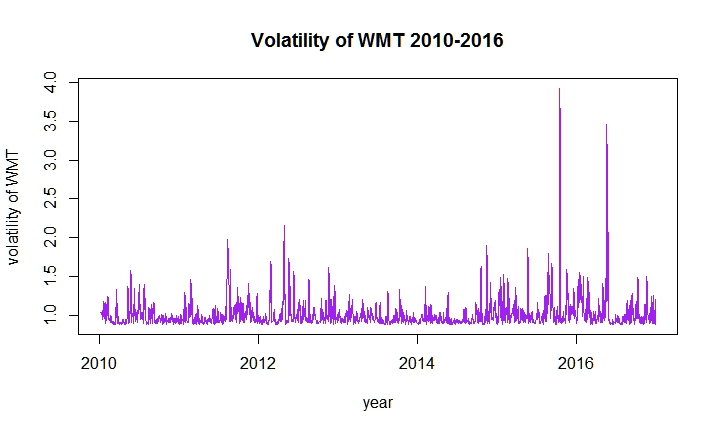
\includegraphics[scale = 0.45]{img/vol_WMT}
\end{minipage}
\begin{minipage}[!htbp]{0.5\linewidth}
\centering
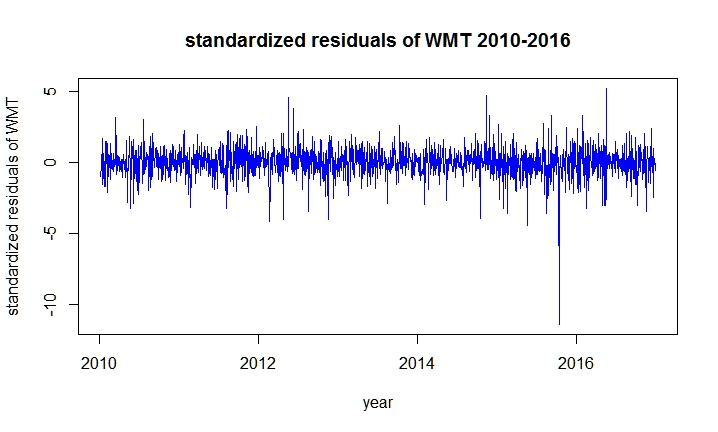
\includegraphics[scale = 0.45]{img/stdr_WMT}
\end{minipage}
\caption{Estimated Volatility Process and Standardized Shocks for WMT}
\label{vol_stdr_wmt}
\end{figure}

Comparing the volatility of the log return series of Amazon and Walmart from 2010 to 2016, we can find that Amazon's volatility is higher and more volatile than that of Walmart. This could probably be explained by two alternative reasons. The first one is that the expectation of Amazon's stock may be stronger than that of Walmart. Stock prices reflect the expected value of a firm. The more frequent the change of the expectation of a firm's future value, the more volatile the firm's stock price and thus the more volatile the stock's return. People hold a stronger expectation of Amazon’s future value and adjust their expectation more often. As a result, the price and return of Amazon's stock is more volatile. Figure \ref{price} shows the stock prices of Amazon and Walmart from 2010 to 2016. We can see that the stock price of Amazon has surged sharply from 2010 to 2017. The stock price of Amazon is below 200 at the beginning of the year 2010 but around 800 at the end of the year 2016. However, the stock price of Walmart has not risen that much. At the beginning of the year 2010, it is between 40 and 50 and at the end of the year 2016, it is around 70. The highest appeared in 2015, which is around 80.

\begin{figure}[!htbp]
\begin{minipage}[!htbp]{0.5\linewidth}
\centering
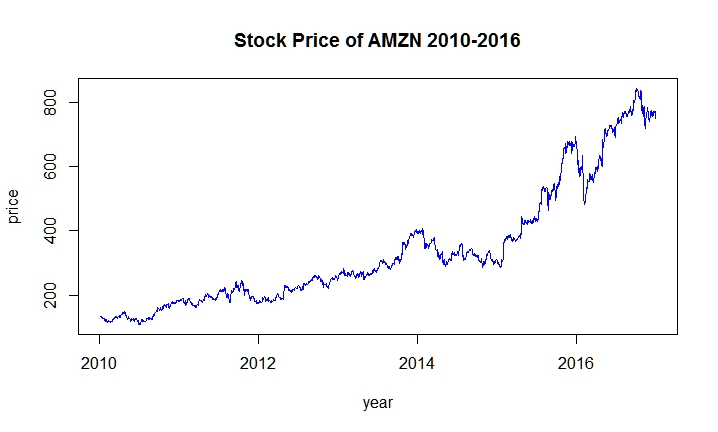
\includegraphics[scale = 0.45]{img/price_AMZN}
\end{minipage}
\begin{minipage}[!htbp]{0.5\linewidth}
\centering
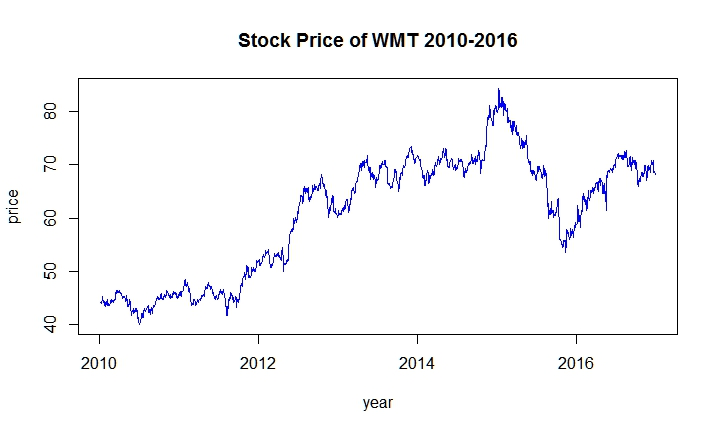
\includegraphics[scale = 0.45]{img/price_WMT}
\end{minipage}
\caption{Stock Prices}
\label{price}
\end{figure}

Another possible reason could be that the market of Amazon's stock is hotter and more prosperous than Walmart's. There may be more participants in the Amazon's stock market. Consequently, the price of Amazon's stock exhibits higher volatility and so does its stock return. However, further observation of the trading volumes of the two stocks contradicts this guess. Figure \ref{volume} shows the trading volumes of the stocks of Amazon and Walmart from 2010 to 2016. We cannot observe a significant larger amount of trading volume in Amazon's stock market. In fact, the trading volume of Walmart's stock is higher than Amazon's in those years.

\begin{figure}[!htbp]
\begin{minipage}[!htbp]{0.5\linewidth}
\centering
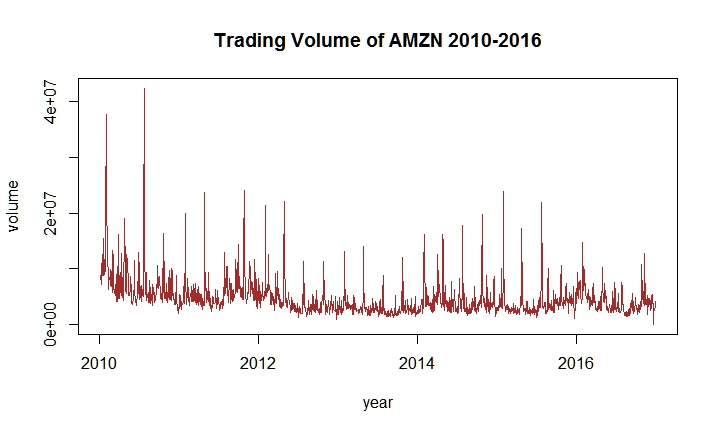
\includegraphics[scale = 0.45]{img/volume_AMZN}
\end{minipage}
\begin{minipage}[!htbp]{0.5\linewidth}
\centering
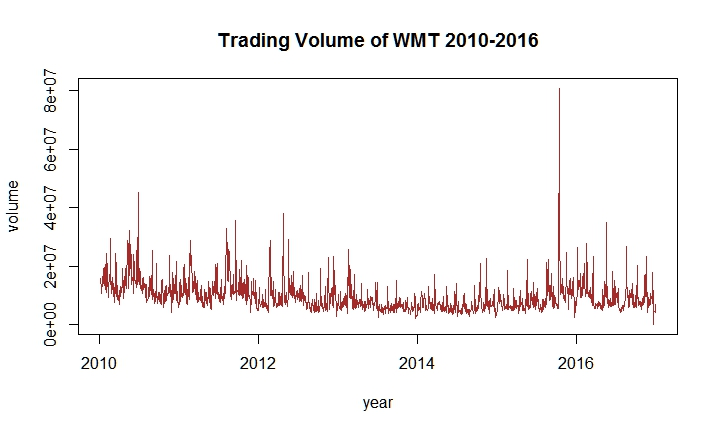
\includegraphics[scale = 0.45]{img/volume_WMT}
\end{minipage}
\caption{Trading Volumes}
\label{volume}
\end{figure}

Both the standardized residual series of Amazon and Walmart look like white noise process, the validity of which are proved by the results of the Ljung-Box tests of the standardized residuals mentioned above.

%%%%%%%%%%%%%%%%%%%%%%   Prediction   %%%%%%%%%%%%%%%%%%%%%%%
\section{Prediction}
Finally, to forecast the volatility of AMZN stock, we can use the volatility equation $\sigma_t^2 = 1.02+0.129a_{t-1}^2+0.637\sigma_{t-1}^2$. The 1-step-ahead forecast is then $\sigma_{h+1}^2 = 1.02+0.129a_h^2+0.637\sigma_h^2$, where $a_h$ is the residual of the mean equation at time $h$ and $\sigma_h$ is obtained from the volatility equation. For multistep-ahead forecasts, we substitute our forecasts recursively. Table \ref{fc_amzn} shows some mean and volatility forecasts for the AMZN stock. Here, the unit for Log Return is in percentage (\%). Similarly, we provide mean and volatility forecasts for the WMT stock in Table \ref{fc_wmt}.

\begin{table}
\caption{Volatility Forecasts for AMZN Stock}
  \centering
\begin{tabular}[!htbp]{c|ccccccc}
\hline Horizon & 1 & 2 & 3 & 4 & 5 & $\infty$ \\ 
\hline Log Return & 0.1367 & 0.1367 & 0.1367 & 0.1367 & 0.1367 & 0.1367 \\
Volatility & 1.8940 & 1.9410 & 1.9763 &  2.0029 & 2.0230 & 2.0876\\
\hline
\end{tabular}
\label{fc_amzn}
\end{table}

\begin{table}
\caption{Volatility Forecasts for AMZN Stock}
  \centering
\begin{tabular}[!htbp]{c|ccccccc}
\hline Horizon & 1 & 2 & 3 & 4 & 5 & $\infty$ \\ 
\hline Log Return & 0.0240 & 0.0240 & 0.0240 & 0.0240 & 0.0240 & 0.0240 \\
Volatility & 0.8920 & 0.9563 & 0.9462 & 0.9608 & 1.0069 & 1.0338\\
\hline
\end{tabular}
\label{fc_wmt}
\end{table}

To make the forecasting results more visualized, Figure \ref{predict} shows the forecasted mean and the corresponding fluctuating range (blue line) based on the forecasted volatility under 5\% significant level for the daily log return of Amazon and Walmart stocks. We also add in the true log returns (red line) from 2017 Jan. 3rd to Jun. 16th, pulled from Wind Terminal. The volatility denotes the conditional standard deviation. As for the stock of Amazon, when the forecast horizon goes to infinity, the return will converge to 0.14\% and the volatility will converge to 2.09. As for the stock of Walmart, when the forecast horizon goes to infinity, the return will converge to 0.02\% and the volatility will converge to 1.03. Obviously, the volatility prediction for AMZN is more efficient because all true values are in the predicted fluctuating range. However, some true values pierce the predicted range, which indicates the prediction is not very accurate.

\begin{figure}[!htbp]
\begin{minipage}[!htbp]{0.5\linewidth}
\centering
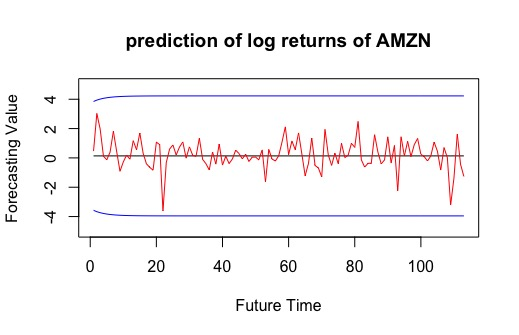
\includegraphics[scale = 0.45]{img/predict_AMZN}
\end{minipage}
\begin{minipage}[!htbp]{0.5\linewidth}
\centering
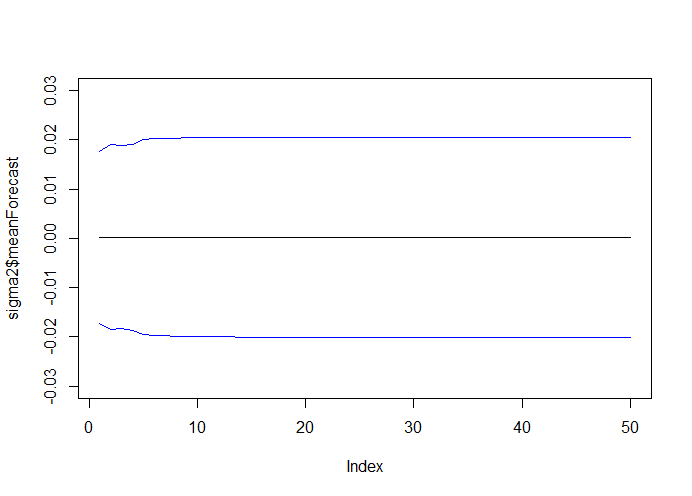
\includegraphics[scale = 0.45]{img/predict_WMT}
\end{minipage}
\caption{Mean (black), True Value (red) and Predicted Volatility (blue) of Log returns}
\label{predict}
\end{figure}

%%%%%%%%%%%%%%%%%%%%%%   Conclusion   %%%%%%%%%%%%%%%%%%%%%%%
\section{Conclusion}
In conclusion, based on our modeling and analysis, both the mean and the volatility of the log return series of Amazon is higher than Walmart’s. The mean reflects the average return and the volatility reflects the risk of holding the stock. This result is consistent with our common sense, higher return is accompanied by higher risk. 
With the rapid development of e-commerce, the operating income of Amazon has increased for three years so far. By contrast, the operating income of Walmart is not as good as Amazon’s. As a traditional physical retail store, Walmart bears higher operating cost than Amazon, the online retail hegemony nowadays. 

Recently, the market value of Amazon’s stock is almost twice as large as Walmart’s. And there is a huge potential that the stock price of Amazon continues to rise in the following years. Amazon has been continuously reducing its logistics costs, which will effectively raise its operating profit. With the introduction of cloud computing service, Amazon is providing customers with more and more attractive and powerful service at lower price. Besides, Amazon is expected to generate more profit by its video service and business in more various fields. But Walmart is not waiting to be left behind. It has exerted great efforts in reversing the situation. In 2016, Walmart purchased the famous e-commerce start-up company, Jet.com in order to acquire more talents in e-commerce. Attaching more importance in e-commerce may help Walmart become more competitive.  

The bugle has sounded. The battle between Amazon and Walmart has already started. Who will be the winner still remains unclear. So just wait and see.

\begin{thebibliography}{99}
\bibitem{1} 
Lieber, Ethan and Chad Syverson. 
\textit{Online vs Offline Competition}. 
The Oxford Handbook of the Digital Economy, 2012.
\begin{CJK}{UTF8}{gkai}
\bibitem{2}
亚马逊市值为何是沃尔玛市值的两倍 \\
http://stock.eastmoney.com/news/1582,20170407726877851.html
\bibitem{3}
亚马逊和沃尔玛的零售巨头之战 多方面比拼谁能胜出?\\
http://tech.ifeng.com/a/20170415/44573838\_0.shtml
\end{CJK}
\end{thebibliography}

\end{document}
